\section{Le Q-Learning}

\subsection{Qu'est-ce que le Q-Learning ?}

L'objectif du $Q$-Learning est de permettre à un agent (notre IA) d'évoluer efficacement dans un environnement (par exemple un jeu). Pour cela, on utilise un système de
récompense. Dans un état donné, l'IA choisit l'action qui lui rapporte le plus de récompense. Néanmoins, on ne veut pas que notre IA choisisse une action parce qu'elle
lui offre une récompense immédiatement. L'IA doit prendre en compte les récompenses qu'elle obtiendrait plus tard en effectuant certaines actions. Cette 
caractéristique du $Q$-Learning permet l'établissement de stratégies.

Pour pouvoir suivre ces stratégies, notre IA se donne des récompenses $Q$ (imaginaires) qui reflètent à la fois la satisfaction obtenue immédiatement mais également
la satisfaction que l'on peut espérer obtenir à l'avenir. Il faut alors que notre système de récompense satisfasse l'équation de \textsc{Bellman} : 

\begin{equation}
 Q\left(s,a\right) = r + \gamma \max_{a'} Q\left(s',a'\right)
 \label{eq:bellman}
\end{equation}

Dans l'équation \ref{eq:bellman}, $s$ représente l'état actuel, $a$ l'action choisie, $r$ la récompense obtenue à cet instant et $s'$ l'état dans lequel on arrive
après avoir effectué l'action $a$. Ainsi, la satisfaction obtenue en effectuant l'action $a$ depuis l'état $s$ correspond à la fois à la récompense obtenue immédiatement
ainsi que la meilleure satisfaction que l'on puisse espérer à l'avenir (on recherche un maximum car l'action $a'$ sera choisie par notre agent). $\gamma$ est le facteur
d'actualisation. Il mesure la préférence à obtenir une récompense à l'instant présent plutôt qu'à l'avenir. Pour ne pas que la satisfaction diverge, il faut que $\gamma$
soit plus petit que 1. Plus il est proche de 1, plus le réseau prend en compte des instants éloignés et établit des stratégies sur le long terme. La valeur du facteur
d'actualisation dépend alors de l'environnement dans lequel est plongé notre agent.

Le principe du $Q$-Learning repose sur l'apprentissage autonome par l'IA de ces différentes valeurs de $Q$ (que nous autres humains ne connaissons pas). 
Pour cela, on distingue deux phases.
La phase d'exploration correspond à agir de manière aléatoire sans prendre en compte la satisfaction. Cela permet de découvrir des voies jusqu'à lors inconnues et 
potentiellement trouver de meilleures stratégies que celles connues à cet instant. Puis, lors de l'exploitation, on utilise les valeurs de satisfaction trouvées
pour choisir notre action. Dans les deux cas, on modifie notre réseau en conséquence (l'exploitation permet de préciser les valeurs de la fonction de satisfaction $Q$).
Le taux d'exploration est au début de la partie de 1 : on a aucun a priori sur les actions à choisir donc on essaie aléatoirement pour collecter un maximum d'informations
sur le jeu. Puis à mesure que l'apprentissage progresse, le taux d'exploration diminue. Il n'atteint généralement pas 0, on veut toujours explorer un peu de temps en temps
dans l'espoir de trouver de meilleures stratégies que celles connues. 

Il existe également une autre politique pour l'exploitation. Plutôt que de choisir systématiquement l'action procurant le plus de satisfaction, on peut
établir des probabilités en fonction des satisfactions calculées et choisir notre action selon ces probabilités. Cette politique ne prend pas seulement en compte
l'action qui a le plus de satisfaction mais également les satisfactions de toutes les actions. Néanmoins, dans nos tests sur différents jeux, nous avons conservé
la politique (dite greedy) qui consiste à choisir l'action possédant la plus grande satisfaction.

\subsection{Calculer la fonction Q}

Lorsque l'on joue (exploration ou exploitation), on enregistre les transitions vécues sur lesquelles on réalise l'entraînement. L'apprentissage se passe de la manière
suivante. D'après \ref{eq:bellman}, $r + \gamma \max_{a'} Q\left(s',a'\right)$ est ce que l'on cherche à obtenir et $Q\left(s,a\right)$ correspond à ce que l'on
a effectivement actuellement. On peut alors retrouver une situation d'apprentissage supervisé (un peu particulière car les données d'apprentissage sont calculées par 
le réseau et évoluent à mesure que le réseau évolue).

Ainsi, on peut utiliser la modification suivante en introduisant le taux d'apprentissage $\lambda$ : 
\begin{equation}
 \Delta Q\left(s,a\right) = \lambda\left(r + \gamma \max_{a'} Q\left(s',a'\right) - Q\left(s,a\right)\right)
 \label{eq:modif-bellman}
\end{equation}

Pour chaque transition (constituée d'un état initial, d'une action, d'une récompense et d'un état final), on calcule la valeur voulue pour la fonction $Q$ 
(équation \ref{eq:bellman}, ou simplement $r$ si la partie se termine) puis on applique le changement décrit équation \ref{eq:modif-bellman}.

Pour un espace des états réduits et un nombre d'actions limité, les valeurs de la fonction $Q$ peuvent être stockées dans un tableau et modifiées de la manière
décrite précédemment.

Lors d'un apprentissage, la transition est choisie aléatoirement. En effet, si on apprend sur les transitions dans l'ordre d'apparition, on augmente le poids de la
dernière transition obtenue. Or, puisqu'un faible changement de $Q$-table peut engendrer un important changement de stratégies, on veut éviter ce genre de dépendance,
c'est pourquoi la transition sur laquelle on apprend est choisie aléatoirement dans l'ensemble des transitions obtenues.


\subsection{Jeu des bâtonnets}

Pour tester le $Q$-Learning, on utilise le jeu des bâtonnets. Il y a deux joueurs et douze bâtonnets sur la table. Alternativement, chaque joueur peut prendre
1, 2 ou 3 bâtonnets. Le joueur contraint de prendre le dernier bâtonnet a perdu. Ce jeu a l'avantage d'avoir un petit espace des états. En effet, l'état est entièrement
décrit par le nombre de bâtonnets restants qui est un entier compris entre 1 et 12. Le nombre d'action est également très faible (3). Ainsi ce jeu se prête parfaitement à
l'utilisation d'une $Q$-table pour représenter la fonction $Q$.

On remarque qu'il existe une stratégie imbattable pour gagner une partie. Si vous commencez la partie, il suffit de prendre 3 bâtonnets puis 4-$x$ bâtonnets à chaque coup
où $x$ est le nombre de bâtonnets pris par l'adversaire. Notre objectif est donc que notre IA découvre cette stratégie et s'y tienne. 

Pour tester notre implémentation, nous faisons jouer à notre IA 100 000 parties (pour annuler les fluctuations statistiques) contre un adversaire jouant aléatoirement
(cela permet de comparer les tests lorsque les apprentissages sont faits dans des contextes différents). Le taux d'apprentissage est fixé à 0.1 et le taux d'actualisation
à 0.9, ce qui est faible mais adapté vu que les parties sont très courtes (moins de dix coups). À chaque coup, la probabilité d'être en exploration évolue 
exponentiellement en fonction du nombre de parties jouées. À la $n$-ième partie, la probabilité d'exploration est $0.999^n$. Puisqu'il existe une stratégie gagnante,
on ne peut s'attendre à gagner 100\% des parties car il existe une probabilité ($\frac{1}{54}$) que le joueur aléatoire l'applique. Ainsi, on ne peut espérer 
converger qu'à 98.15\% de victoires. Lors des tests, on est bien sûr constamment en phase d'exploitation, sans entraînement sur les transitions.

Nous avons testé différents contextes d'apprentissage en utilisant différents adversaires. Tout d'abord nous avons appris sur une IA qui apprend en même temps. Puis 
nous avons essayé de reproduire les résultats en apprenant sur un joueur jouant aléatoirement. Enfin, notre IA devra apprendre contre un joueur connaissant et 
appliquant la stratégie gagnante. Dans tous les cas, les tests sont fait contre un adversaire jouant aléatoirement pour pouvoir comparer les résultats.

\begin{figure}[h]
 \centering
 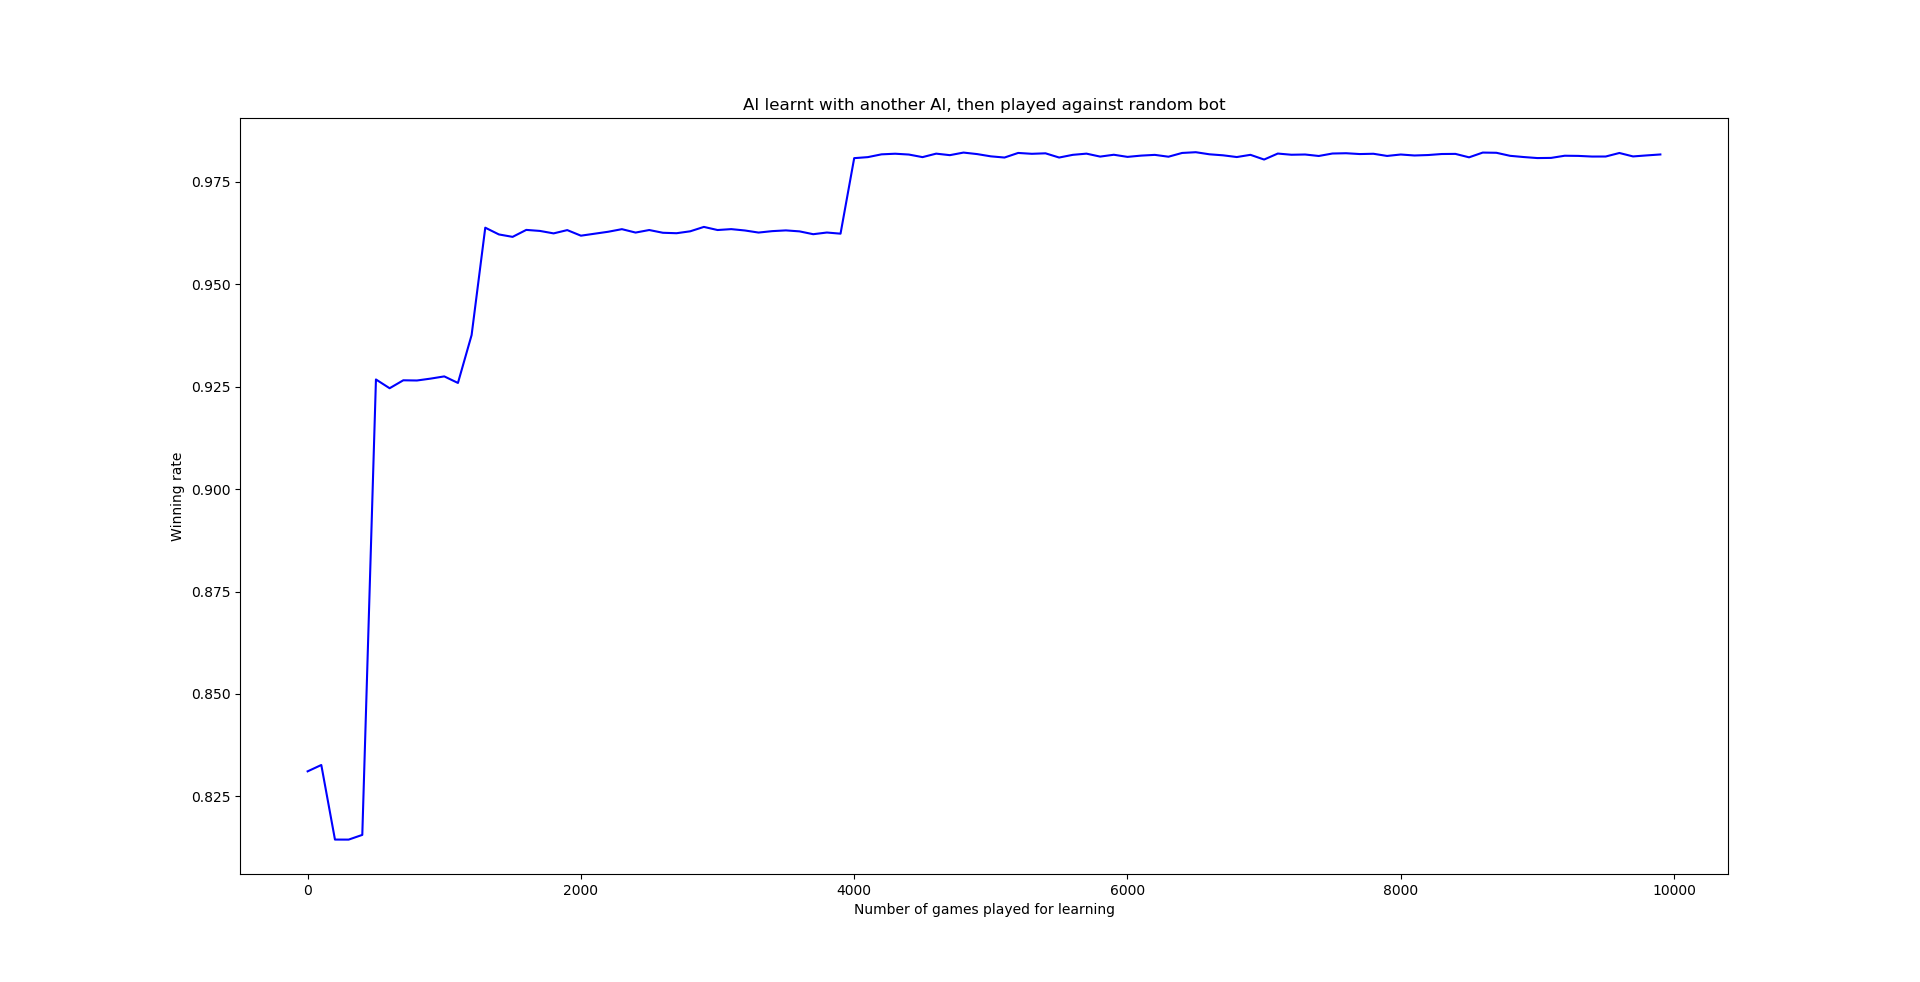
\includegraphics[width = 0.9\textwidth]{img/learnWithAI_testRandom.png}
 \caption{Apprentissage contre une autre IA apprenant en même temps}
 \label{fig:learnWithAI}
\end{figure}

La figure \ref{fig:learnWithAI} nous présente les résultats lorsque notre IA apprend contre une autre IA apprenant également à jouer à ce jeu. On remarque plusieurs choses.
La convergence à 98.15\% ainsi que la $Q$-table nous confirme que notre IA a réussi à apprendre quelle était la stratégie parfaite pour jouer à ce jeu. L'apprentissage 
est donc réussi. On remarque également que la courbe semble être en escalier. Cela provient du fait que pour choisir une action lors de l'exploitation, on choisit celle
avec la meilleure satisfaction mais leurs valeurs respectives n'ont pas plus d'incidence. Ainsi, deux $Q$-table différentes mais ayant la même action préféré à chaque état
auront des taux de victoires similaires. La modification de la $Q$-table n'entraîne pas nécessairement un changement de stratégie, c'est pourquoi on observe ces plateaux.
Pour la même raison, on observe des sauts. Même si deux actions procurent presque la même satisfaction, on choisit toujours celle qui en procure le plus. Ainsi, un faible
changement de la $Q$-table peut entraîner un changement radical dans la stratégie adoptée par notre IA. Ce changement se ressent alors fortement dans le taux de victoires
lorsque l'IA est confrontée au joueur aléatoire. Vu la simplicité du jeu, un nombre raisonnable de parties (quelques milliers) est nécessaire pour comprendre la stratégie,
ce qui s'effectue très rapidement (en quelques minutes).

\begin{figure}[h]
 \centering
 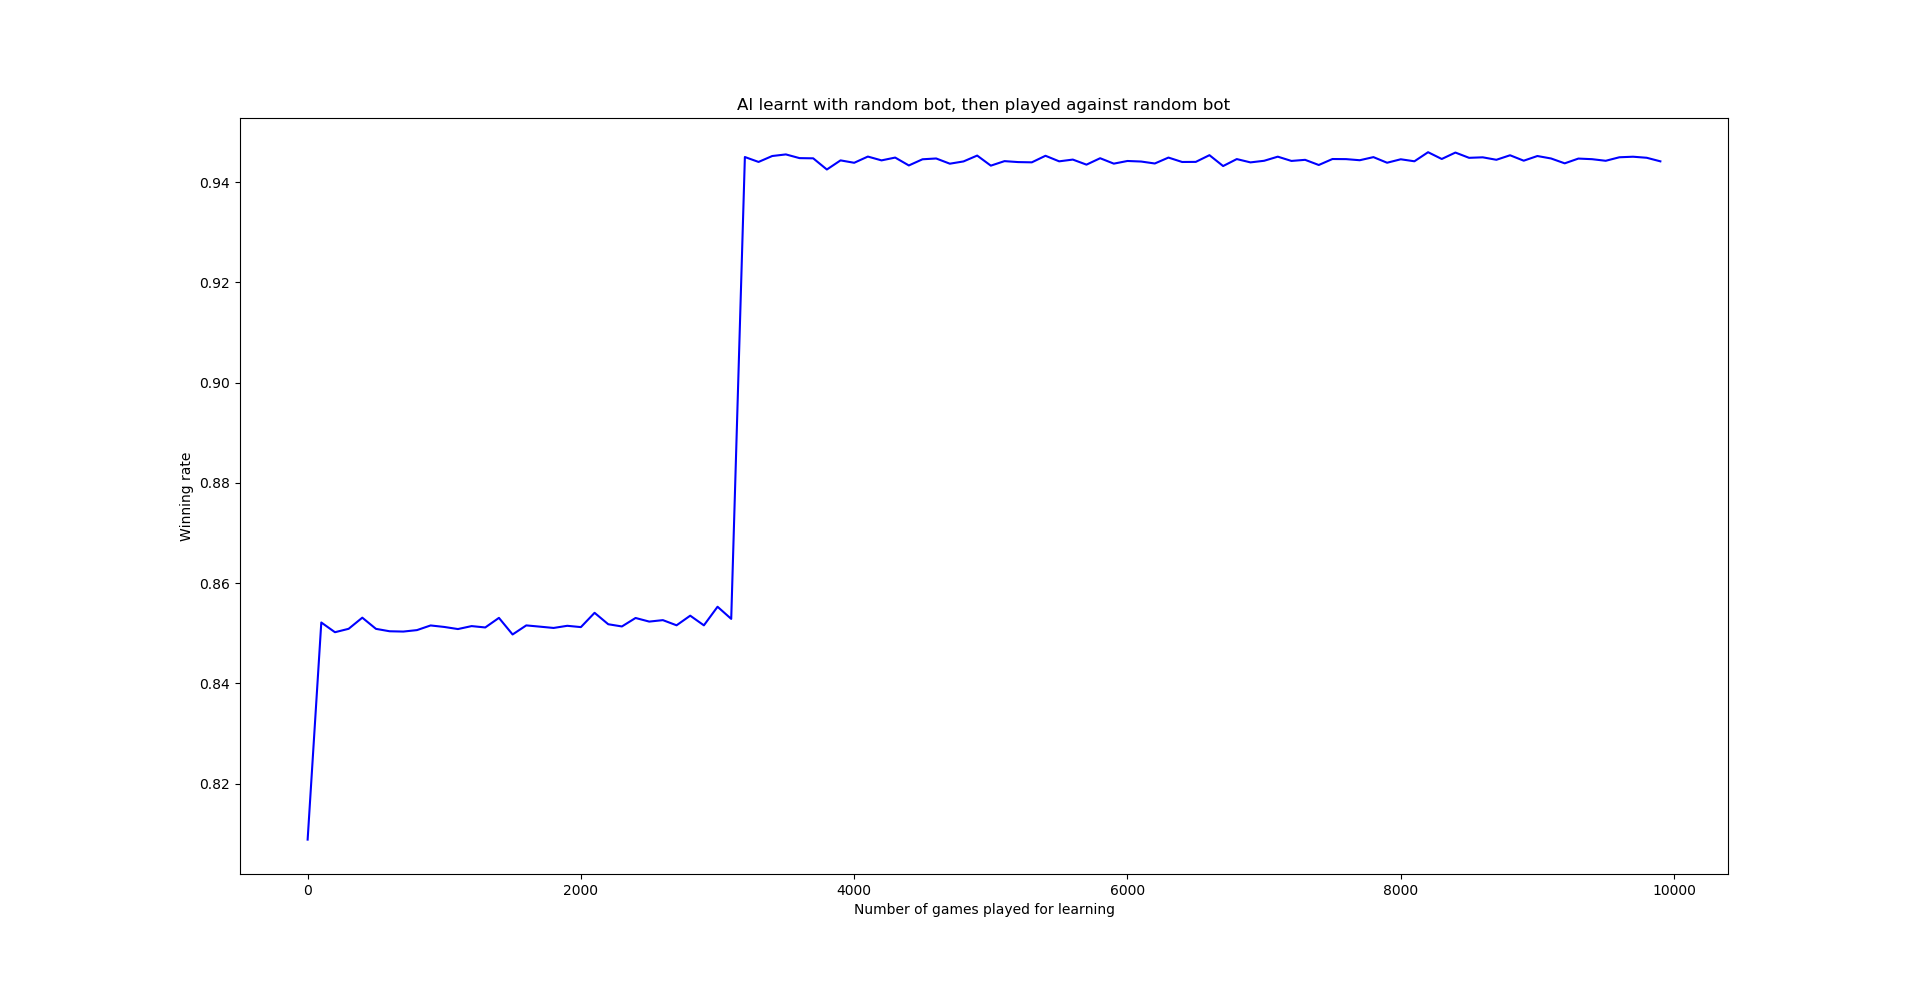
\includegraphics[width=0.9\textwidth]{img/learnRandomly.png}
 \caption{Apprentissage contre un joueur jouant aléatoirement}
 \label{fig:learnRandomly}
\end{figure}

La figure \ref{fig:learnRandomly} nous présente les mêmes résultats lorsque l'IA apprend sur un joueur sélectionnant son action aléatoirement. On remarque que la convergence
est plus lente et imparfaite (à 94\% de victoires environ). Cela provient du fait que le joueur adverse joue aléatoirement. Ainsi, même si notre IA réalise un mauvais 
coup (contraire à la stratégie), il existe une probabilité que le joueur adverse n'en profite pas pour appliquer la stratégie mais redonne l'avantage à notre IA. Cela
signifie alors que notre IA surestime la satisfaction de certains coups. Elle n'a donc pas compris la stratégie car le joueur adverse, trop complaisant, ne la
sanctionnait pas lorsqu'elle choisissait une mauvaise action. On en conclut qu'il faut proscrire l'apprentissage contre un joueur jouant aléatoirement.

\begin{figure}[h]
 \centering
 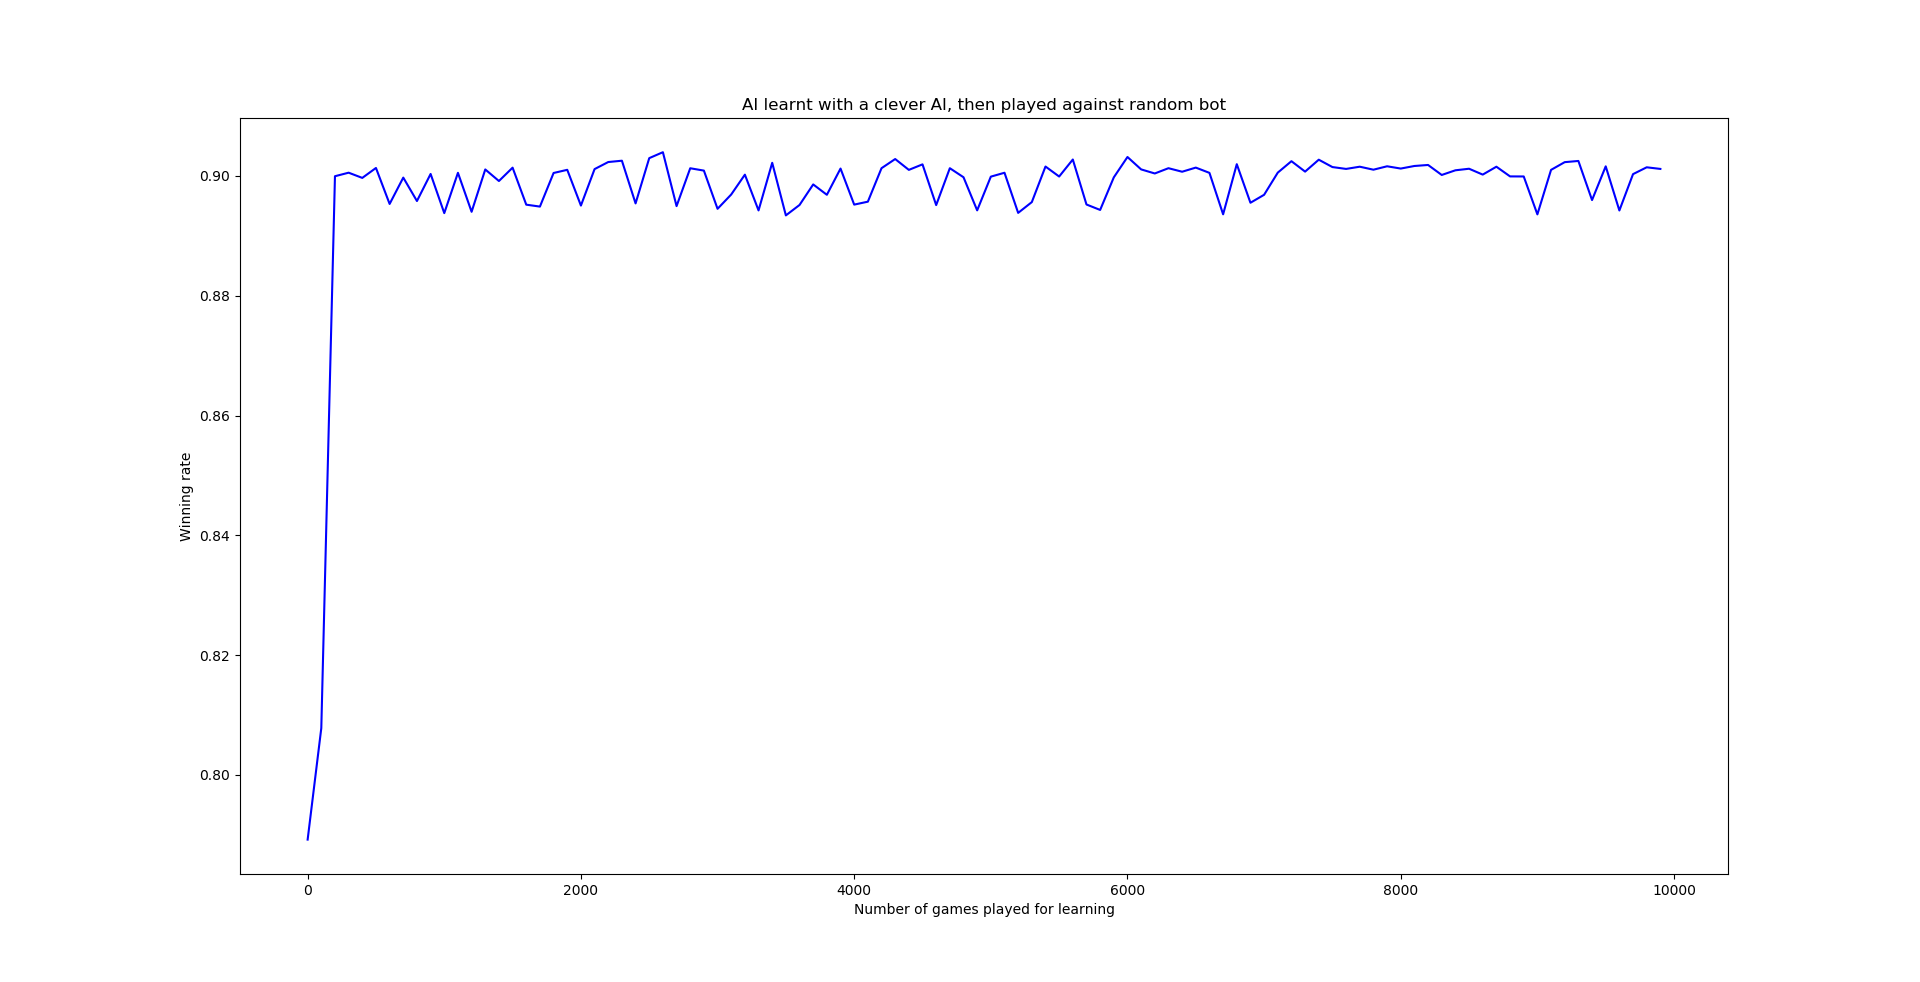
\includegraphics[width=0.9\textwidth]{img/learnWithGod.png}
 \caption{Apprentissage contre un joueur appliquant la stratégie gagnante}
 \label{fig:learnWithGod}
\end{figure}

Enfin, la figure \ref{fig:learnWithGod} reprend le même jeu mais notre IA apprend contre un joueur ayant compris la stratégie gagnante et l'appliquant systématiquement.
On observe deux résultats importants : la convergence est plus rapide mais imparfaite (environ 90\% de victoires). La rapidité de la convergence provient du fait
que le joueur adverse sanctionne instantanément tout coup contraire à la stratégie (car il joue parfaitement). Ainsi, notre IA comprend rapidement que certains coups 
ne doivent pas être joués. L'imperfection de la convergence provient également du fait que l'adversaire applique la stratégie. Il y a donc certains états dans lequel
il ne veut surtout pas se retrouver car cela serait à l'avantage de notre IA. Cette tendance à éviter certains états empêche notre IA d'explorer l'ensemble de l'espace 
des états. Elle ne peut donc pas trouver quelle est la meilleure stratégie car une partie de l'espace des états demeure inconnue.

La rapidité de convergence est néanmoins intéressante. On peut alors imaginer commencer l'apprentissage contre un joueur très compétent pour vite cerner les quelques
principes fondamentaux du jeu, puis finir l'apprentissage contre un joueur apprenant en même temps pour pouvoir explorer la totalité de l'espace des états et continuer
d'apprendre relativement efficacement. Néanmoins, la simplicité du jeu en question joue probablement en faveur de cette convergence. On peut se demander si cette 
caractéristique demeurerait sur un jeu plus complexe où l'espace des états est beaucoup plus important.


\subsection{Le labyrinthe}

On se place sur un plan quadrillé. Chaque case contient une récompense (positive, négative ou nulle). L'objectif est d'atteindre l'arrivée avec le plus de satisfaction.
Atteindre l'arrivée est une condition de victoire (le jeu s'arrête). Certaines cases, en plus de procurer une récompense négative, peuvent également provoquer une 
défaite instantanée. 

\begin{figure}[h]
 \centering
 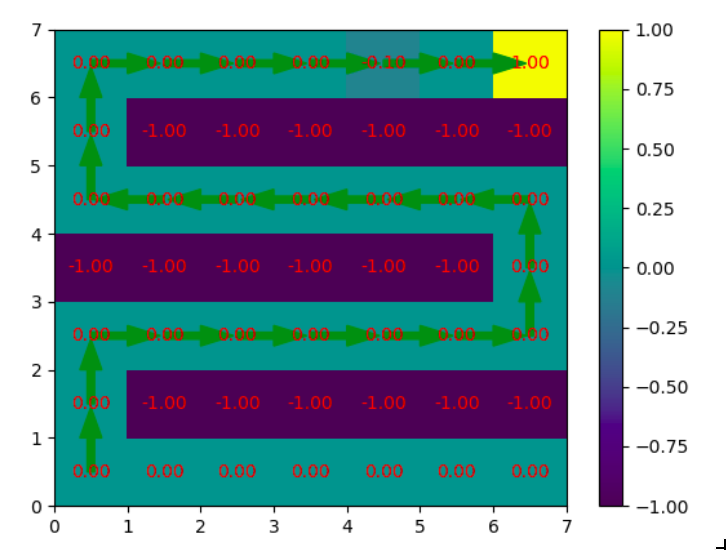
\includegraphics[width = 0.5\textwidth]{img/labyrinthe.png}
 \caption{Chemin choisi par l'IA lorsque confrontée à un labyrinthe donné}
 \label{fig:labyrinthe}
\end{figure}

La figure \ref{fig:labyrinthe} représente le chemin choisi par l'IA lorsque celle-ci est confrontée à un labyrinthe particulier, en serpentin. On remarque que l'IA choisit
un chemin qui l'amène à l'arrivée, tout en maximisant les récompenses obtenues sur le chemin. L'apprentissage sur d'autres labyrinthes générés aléatoirement
font également apparaître un apprentissage réussi et donc une capacité à atteindre la sortie du labyrinthe.

